%% Phase 4 research paper -- Springer Nature LaTeX template (sn-jnl).
%% Compile inside the "Springer Nature LaTeX Template" (Overleaf), which supplies sn-jnl.cls and
%% the bibliography styles. Compiler: pdfLaTeX. Bibliography: references.bib (BibTeX).
\documentclass[pdflatex,sn-mathphys-num]{sn-jnl}

\usepackage{graphicx}%
\usepackage{multirow}%
\usepackage{amsmath,amssymb,amsfonts}%
\usepackage{amsthm}%
\usepackage{mathrsfs}%
\usepackage[title]{appendix}%
\usepackage{xcolor}%
\usepackage{textcomp}%
\usepackage{manyfoot}%
\usepackage{booktabs}%
\usepackage{algorithm}%
\usepackage{algorithmicx}%
\usepackage{algpseudocode}%
\usepackage{array}%
\usepackage{url}%

\newcolumntype{L}[1]{>{\raggedright\arraybackslash}p{#1}}
\newcolumntype{C}[1]{>{\centering\arraybackslash}p{#1}}
\newcommand{\Fone}{F\textsubscript{1}}
\newcommand{\pub}{\textsuperscript{*}}

\raggedbottom

\begin{document}

\title[Website Fingerprinting on Encrypted DNS, Revisited]{Does Encrypted DNS Still Hide Visited Websites? Reproducing a 2020 Fingerprinting Attack and Testing It from Pakistan Against Deployed Padding}

\author*[1]{\fnm{Muhammad} \sur{Kaif}}\email{i240071@isb.nu.edu.pk}
\author[1]{\fnm{Samran} \sur{Ahmad}}\email{i243013@isb.nu.edu.pk}
\affil*[1]{\orgname{National University of Computer and Emerging Sciences (FAST-NUCES)}, \orgaddress{\city{Islamabad}, \country{Pakistan}}}

\abstract{DNS over HTTPS (DoH) encrypts the names a browser resolves, yet the sizes and timing of encrypted records still reveal the visited website. The best-known attack of this kind (Siby et al., NDSS 2020) was measured on 2018--19 traffic and never re-measured, although browsers, TLS and resolver padding have since changed. This study reproduces it on its released data under a tolerance fixed in advance; collects PK-DoH-2026, 1,998 Chrome page loads of 100 websites (50 Pakistani) in Pakistan against a padding (Cloudflare) and a non-padding (Quad9) resolver; audits the padding of 11 public resolvers; and proposes a fused random forest over size n-grams, burst statistics and timing. The reproduction matches the published macro-\Fone{} (0.893 against 0.898; equivalence test $p<0.001$), and five of six published configurations are within tolerance, one under a corrected reading of the setup. In 2026 the attack identifies sites with macro-\Fone{} 0.948 against the unpadded resolver but 0.342 against the padded one, and 2018--19 models are at chance on 2026 traffic. Only one of the 11 resolvers always pads; Cloudflare and Google pad DoH replies only when the client pads its query. The fused model is the only method within 0.025 of the best on both resolvers (0.444 padded, 0.923 unpadded); under padding it gains 0.102 (+30\%) over the original attack (Wilcoxon $p=0.002$). Encrypted DNS therefore still leaks the visited site; padding helps only where client and resolver both apply it, and even then does not reduce the attack to chance.}

\keywords{website fingerprinting, DNS over HTTPS, EDNS(0) padding, traffic analysis, reproducibility, privacy measurement}

\maketitle

%% ===================================================================== 1
\section{Introduction}\label{sec:intro}

DNS over HTTPS (DoH)~\cite{rfc8484} and DNS over TLS (DoT)~\cite{rfc7858} encrypt the names a browser resolves; thousands of public resolvers now offer them~\cite{bielefeld2026}, and Chrome supports DoH natively. Encryption hides each message's content but not the traffic's shape: an observer between user and resolver, such as an ISP or a Wi-Fi operator, still sees how many encrypted records a page load produces, their sizes and their timing. Siby et al.~\cite{siby2020} showed in 2020 that this shape identifies the visited page (macro-\Fone{} 0.898 over 1,500 pages), and that EDNS(0) padding to 468-byte blocks~\cite{rfc7830,rfc8467} still left 0.430.

Since then, browsers have moved to TLS~1.3~\cite{rfc8446}, Chrome pads its own queries (Section~\ref{sec:results}), and attacks have moved to newer transports~\cite{zhang2026dohfuse,salari2025odoh,mouregarrido2026,csikor2025,rfc9250}. Three questions remain open: whether the 2020 results can be reproduced from the released artefact; whether models built in one region and era transfer to users elsewhere, years later, given that recent measurements come from a single country~\cite{mouregarrido2026,salari2025odoh,csikor2025}; and how much the padding a user actually receives reduces the attack, which has been surveyed~\cite{li2025unraveling} or simulated~\cite{gong2026wfcat,jiang2026camouflage} but never tied to attack accuracy under otherwise identical conditions. The contributions of this work are:
\begin{itemize}
\item a \textbf{pre-registered reproduction} of Siby et al.~\cite{siby2020} (within 0.005 \Fone{}; five of six configurations within tolerance) documenting three artefact--paper mismatches;
\item \textbf{PK-DoH-2026}, to the authors' knowledge the first encrypted-DNS fingerprinting dataset from South Asia (1,998 page loads, 100 sites, 50 Pakistani);
\item a \textbf{padding audit of 11 resolvers} and a single-factor contrast: deployed padding cuts macro-\Fone{} from 0.948 to 0.342;
\item a \textbf{fused random forest}, the only method within 0.025 of the best on both resolvers (+0.102 over the original attack under padding);
\item a \textbf{cross-era transfer matrix and recovery curves}: 2018--19 models are at chance on 2026 traffic.
\end{itemize}
Sections~\ref{sec:related}--\ref{sec:setup} cover related work, methodology and setup; Sections~\ref{sec:results}--\ref{sec:ablation} report the results, the comparison with the base papers and the state of the art, and the ablations; Section~\ref{sec:discussion} discusses the findings and Section~\ref{sec:conclusion} concludes.

%% ===================================================================== 2
\section{Related Work}\label{sec:related}

\paragraph{Fingerprinting encrypted DNS.} Siby et al.~\cite{siby2020} classify n-grams of signed TLS record and burst sizes with a random forest~\cite{breiman2001rf}; the attack degrades across locations (16--27\%), and padding reduces but does not remove it~\cite{bushart2020}. Later work followed newer transports: DoHFuse~\cite{zhang2026dohfuse} attacks DoH/3 with timing only (95.48\% on 100 sites; its size-only control still reaches 67.39\% on 449 sites), Salari et al.~\cite{salari2025odoh} attack Oblivious DoH and lose 9\% on an unseen US location, and Csikor et al.~\cite{csikor2025} and Moure-Garrido et al.~\cite{mouregarrido2026} attack DNS over QUIC, the latter with burst statistics and 53.2--81.0\% cross-node transfer within one country. Li et al.~\cite{li2025unraveling} surveyed padding across public DoH resolvers and built a padding-resilient timing attack.

\paragraph{Ecosystem, drift and realism.} Resolver surveys omit padding~\cite{bielefeld2026}; IP addresses alone leak sites, and CDN mappings are regional~\cite{ahmad2026ipv6}; defences can be priced by their overhead~\cite{jimenez2025forgery}. Fingerprints drift with time and browser versions~\cite{shusterman2026}, but a few traces per site recover much of the loss~\cite{zhao2026traverse}; timing features survive size-only defences~\cite{gong2026wfcat}; and realistic traffic lowers accuracy~\cite{deng2026,jansen2026gtt23}.

\paragraph{Positioning.} Table~\ref{tab:coverage} summarises the key studies; this work is the only one covering every dimension except newer transports.

\begin{table}[t]
\caption{Coverage of key related work (\checkmark: measured, not only discussed).}\label{tab:coverage}
\scriptsize\setlength{\tabcolsep}{2pt}
\begin{tabular*}{\textwidth}{@{\extracolsep\fill}L{0.18\textwidth}C{0.07\textwidth}C{0.09\textwidth}C{0.09\textwidth}C{0.08\textwidth}C{0.10\textwidth}C{0.09\textwidth}C{0.09\textwidth}@{}}
\toprule
Study & DoH/2 & Newer transport & Outside US/EU & Time or era & Padding as deployed & Repro\-duction & Variance \\
\midrule
Siby et al. 2020~\cite{siby2020} & \checkmark & -- & \checkmark & \checkmark & partly & -- & \checkmark \\
Moure-Garrido et al. 2026~\cite{mouregarrido2026} & -- & DoQ & -- & -- & -- & -- & \checkmark \\
DoHFuse 2026~\cite{zhang2026dohfuse} & -- & DoH/3 & -- & -- & observed & -- & \checkmark \\
Salari et al. 2025~\cite{salari2025odoh} & -- & ODoH & -- & \checkmark & -- & -- & -- \\
Li et al. 2025~\cite{li2025unraveling} & \checkmark & -- & -- & -- & surveyed & -- & -- \\
Shusterman et al. 2026~\cite{shusterman2026} & -- & -- & -- & \checkmark & -- & -- & -- \\
\textbf{This work} & \checkmark & -- & \checkmark & \checkmark & \checkmark & \checkmark & \checkmark \\
\botrule
\end{tabular*}
\end{table}

%% ===================================================================== 3
\section{Proposed Methodology}\label{sec:method}

\paragraph{Problem formulation and architecture.} A passive adversary observes the encrypted connection between a browser and a DoH resolver with a known IP address. For one page visit it records a trace $x=((s_1,t_1),\dots,(s_n,t_n))$, where $s_i\in\mathbb{Z}\setminus\{0\}$ is the length of the $i$-th TLS record (positive client-to-resolver, negative resolver-to-client) and $t_i$ its capture time. In the closed world the site belongs to $\mathcal{Y}=\{1,\dots,K\}$; a classifier $f$ maps $x$ to class probabilities and predicts $\hat{y}=\arg\max_k f_k(x)$. Performance is macro-\Fone{}, $\frac{1}{K}\sum_k 2P_kR_k/(P_k+R_k)$, with $P_k$ and $R_k$ the precision and recall for site $k$; chance is $1/K$. Figure~\ref{fig:pipeline} shows three tracks feeding one pipeline: Track~A reproduces the 2020 attack (RQ1), Track~B collects PK-DoH-2026 and tests transfer (RQ2), and Track~C audits padding (RQ3) and selects the resolvers for Track~B.

\begin{figure}[t]
\centering
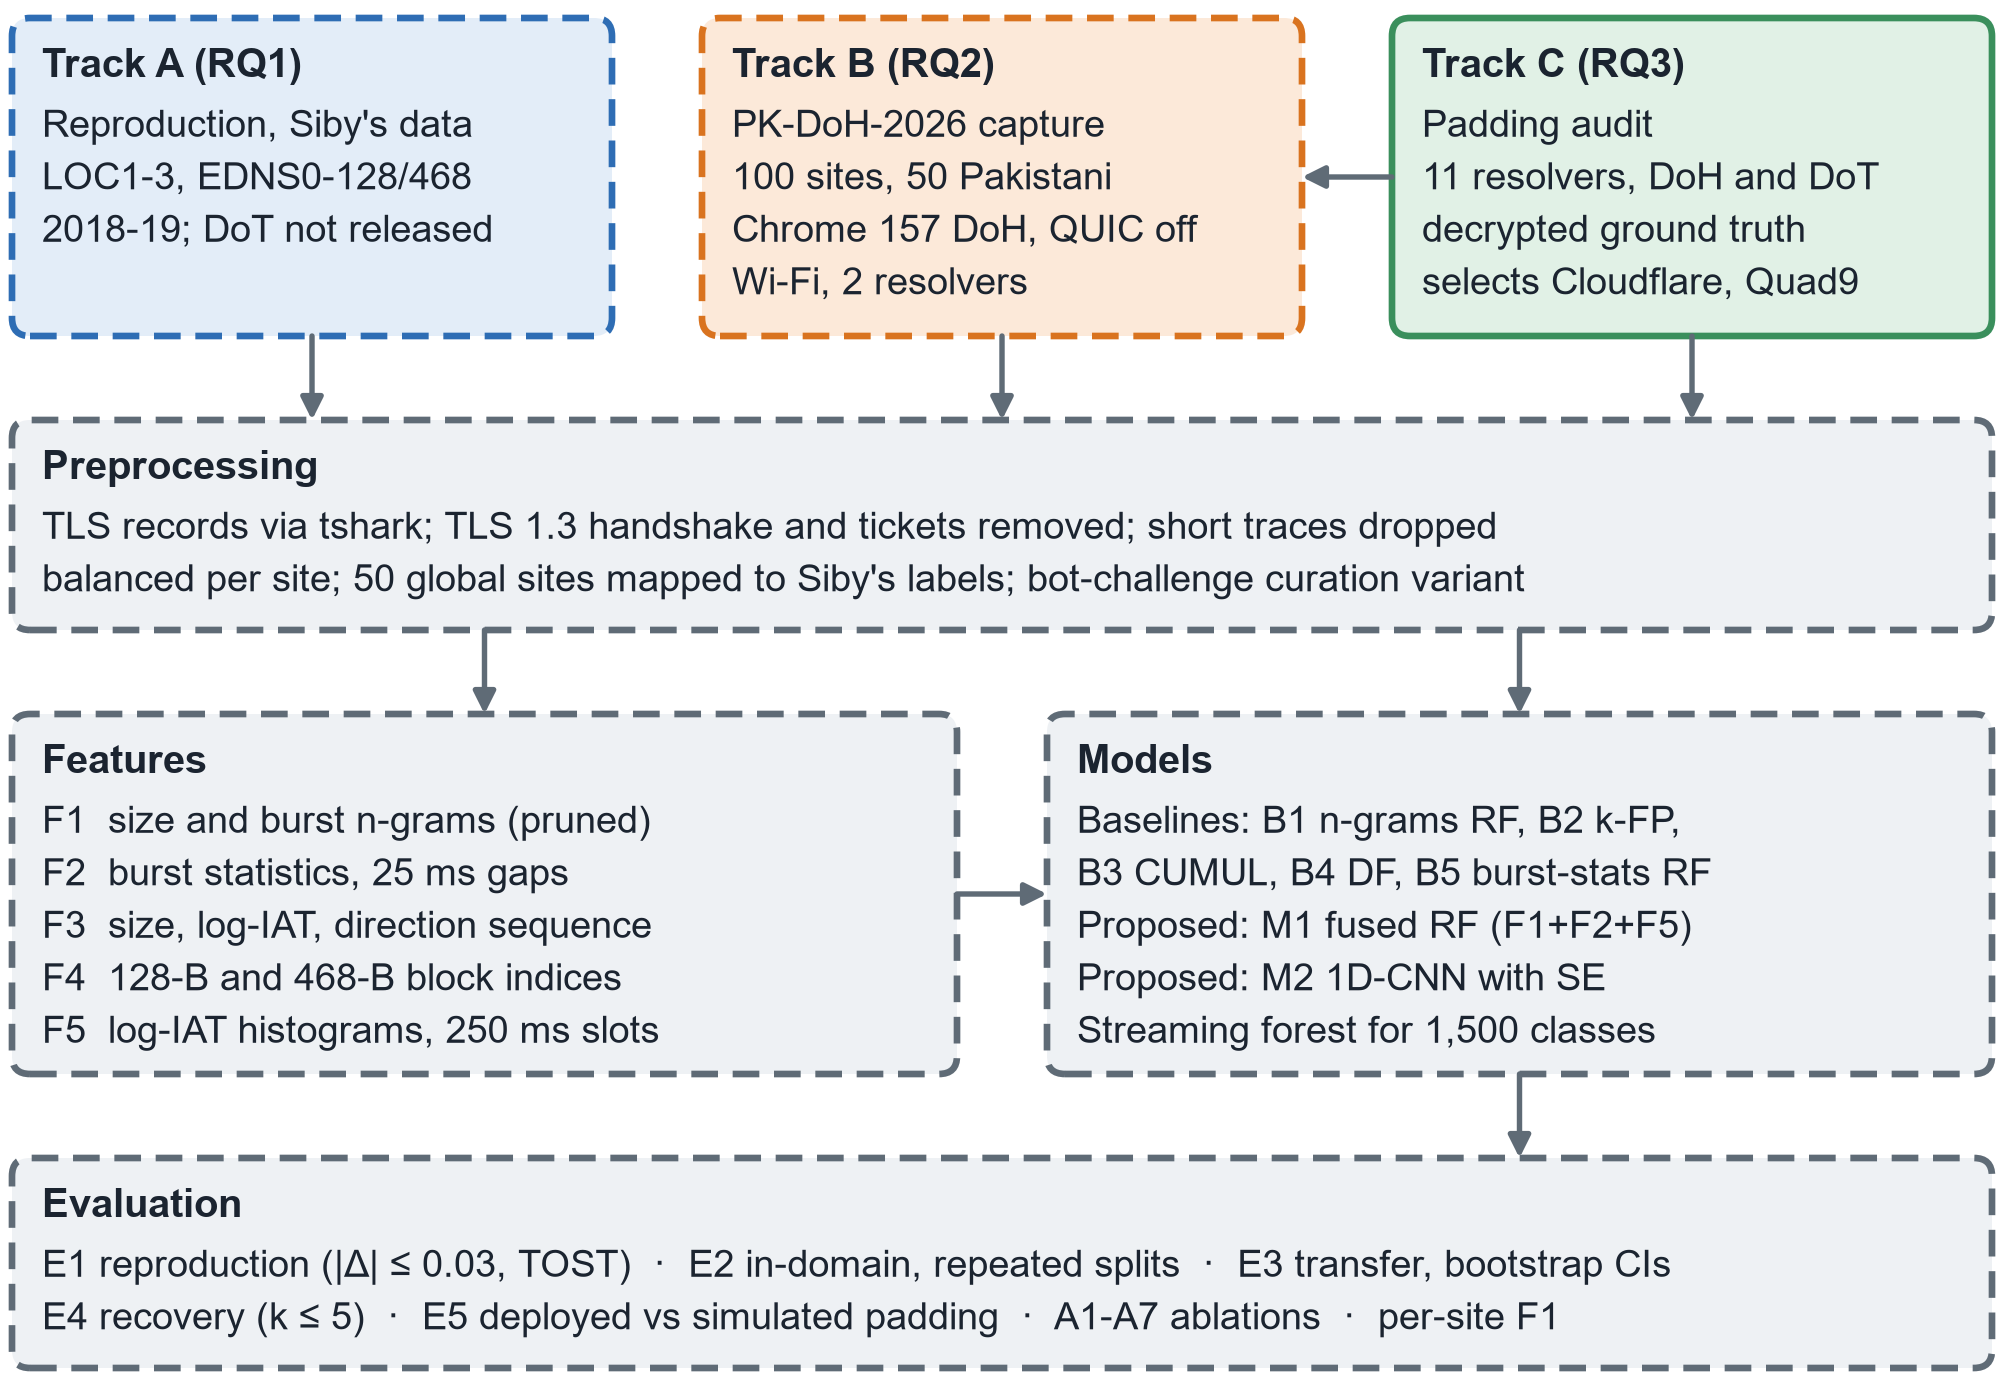
\includegraphics[width=0.92\textwidth]{figures/fig1_pipeline.png}
\caption{Architecture of the study. Dashed borders mark components changed from the planned design.}\label{fig:pipeline}
\end{figure}

\paragraph{Capture and TLS~1.3 alignment.} Each visit follows Algorithm~\ref{alg:extract}. In TLS~1.3~\cite{rfc8446} the certificate chain, the client \emph{Finished} message and the session tickets travel as encrypted records, which would add about 2~kB of site-independent records to the start of every 2026 trace. Removing them makes a 2026 trace start at the first DNS exchange, as a 2018 TLS~1.2 trace does; to the authors' knowledge this mismatch has not been addressed before.

\begin{algorithm}[t]
\caption{Per-visit capture and trace extraction}\label{alg:extract}
\begin{algorithmic}[1]
\Require site $u$, resolver address $a$, timeout $T=30$\,s, idle time $\delta=5$\,s
\State fresh browser profile with Secure DNS forced to DoH server $a$; QUIC disabled
\State capture packets to and from $a$:443; load \texttt{http://}$u$ (abort after $T$); wait $\delta$; stop
\For{each TLS connection $c$}
  \State drop encrypted records of $c$ up to and including the client's first one (handshake)
  \State drop server records of $c$ of at most 300 bytes before the first request (tickets)
\EndFor
\State \Return $x=((s_i,t_i))_i$ in time order, with label $u$
\end{algorithmic}
\end{algorithm}

\paragraph{Features.} A \emph{burst} is a maximal run of records in one direction; if $I_j$ is the set of its record indices, its signed size is $b_j=\sum_{i\in I_j}s_i$. \textbf{F1}~\cite{siby2020}: counts of uni- and bi-grams of $(s_i)$ and $(b_j)$ seen in at least three training traces. \textbf{F2}~\cite{mouregarrido2026}: 24 statistics of bursts also split at gaps above $\tau=25$\,ms (counts, bytes, duration, Gini concentration, gravity centre). \textbf{F3}: the first 200 records as size, log inter-arrival time and direction channels. \textbf{F4}: F1 on block indices $\operatorname{sign}(s_i)\lceil|s_i|/\beta\rceil$ for a padding block size $\beta\in\{128,468\}$ bytes. \textbf{F5} (after~\cite{gong2026wfcat}): per 250-ms slot (20 slots) and direction, an 8-bin histogram of log inter-arrival times (320 values).

\paragraph{M1: fused random forest (proposed).} M1 concatenates three views, $\phi(x)=[\phi_{\mathrm{F1}}(x);\phi_{\mathrm{F2}}(x);\phi_{\mathrm{F5}}(x)]$, and trains $N_T=100$ fully grown trees. Each split minimises the Gini impurity $1-\sum_k p_k^2$, where $p_k$ is the share of class $k$ in the node, over $\sqrt{d}$ randomly chosen features, $d$ being the dimension of $\phi(x)$. The forest averages the trees' class distributions, $f(x)=\frac{1}{N_T}\sum_{b=1}^{N_T} f_b(x)$, where $f_b$ is the $b$-th tree. Padding hides sizes but not the number, grouping and pacing of exchanges, so the forest can use F1 when sizes are informative and F2 and F5 when they are padded. F5 is kept as planned, although it adds nothing beyond F1 and F2 at this sample size (Section~\ref{sec:ablation}).

\paragraph{M2: 1D-CNN with squeeze-and-excitation (proposed).} Three convolutional blocks (32, 64 and 128 channels, kernel 5), each followed by a squeeze-and-excitation layer~\cite{hu2018se}, take F3 as input. Training minimises the label-smoothed cross-entropy $\mathcal{L}=-\sum_k q_k\log f_k(x)$, with $q_k=(1-\alpha)\mathbb{1}[k=y]+\alpha/K$ and $\alpha=0.05$, using AdamW~\cite{loshchilov2019adamw}.

\paragraph{Reproduction criterion, padding model and scalability.} For each configuration, $\Delta=\mathrm{F1}_{\mathrm{rep}}-\mathrm{F1}_{\mathrm{pub}}$, the reproduced minus the published macro-\Fone{}. A result counts as \emph{reproduced} if $|\Delta|\le\varepsilon=0.03$ and \emph{partly reproduced} if $|\Delta|\le0.10$; this rule was fixed before any code was run, and 0.03 is ten times the standard deviation of the main configuration in~\cite{siby2020} ($\pm0.003$). A TOST equivalence test~\cite{schuirmann1987tost} checks $H_1:|\Delta|<\varepsilon$. Padding with block size $\beta$ is simulated as $s_i'=\operatorname{sign}(s_i)\,\beta\lceil|s_i|/\beta\rceil$; perfect padding sets every record to 825 bytes; the byte overhead is $O=\sum|s_i'|/\sum|s_i|-1$. With 1,500 classes a 100-tree forest needs about 100~GB of memory, so Algorithm~\ref{alg:forest} (Appendix~\ref{app:extra}) grows the same trees in batches and frees them after scoring, giving an identical output in bounded memory.

\paragraph{Changes from the plan.} The planned methodology received no external feedback; the changes made during implementation (Python~3 port, TLS~1.3 alignment, streaming forest, 10 instead of 30 traces per site, a resolver contrast in place of the uncollected mobile network, $k\le5$, 250-ms slots) are listed in Table~\ref{tab:deviations} (Appendix~\ref{app:extra}).

%% ===================================================================== 4
\section{Experimental Setup}\label{sec:setup}

\paragraph{Datasets.} Table~\ref{tab:datasets} lists the data. The published sets~\cite{siby2020,sibycode} are LOC1--3 (2018) and EDNS0-128/468 (2019). The paper describes the padded sets as 700 pages $\times$ 60 samples, but only 700 of the 1,500 released EDNS0-468 pages have 60 or more samples, so those 700 are evaluated. PK-DoH-2026 has 100 labels: 50 global sites from Siby's list, mapped to its class indices so that the eras share labels, and 50 Pakistani sites (news, e-commerce, government, banking, education, telecom). Ten rounds per site and resolver were collected in headless Chrome~157 over residential Wi-Fi in Pakistan in November 2026 by eight workers, each bound to one of four identically padding anycast addresses of Cloudflare or Quad9.

\begin{table}[t]
\caption{Datasets. Len.: median records per trace; CV: median within-site coefficient of variation of length~\cite{jansen2026gtt23}. CF: Cloudflare. \pub{} Released by~\cite{siby2020}; all statistics computed in this work.}\label{tab:datasets}
\scriptsize\setlength{\tabcolsep}{3pt}
\begin{tabular*}{\textwidth}{@{\extracolsep\fill}lllllrrr@{}}
\toprule
Dataset & Place & Year & Resolver / client & Padding & Traces & Len. & CV \\
\midrule
LOC1\pub & Lausanne & 2018 & CF / cloudflared & none & 415,562 & 59 & 0.24 \\
LOC2\pub & Leuven & 2018 & CF / cloudflared & none & 311,948 & 54 & 0.05 \\
LOC3\pub & Singapore & 2018 & CF / cloudflared & none & 154,933 & 77 & 0.03 \\
EDNS0-128\pub & Lausanne & 2019 & CF & 128-B & 132,922 & 76 & 0.05 \\
EDNS0-468\pub & Lausanne & 2019 & CF via proxy & 468-B & 83,794 & 68 & 0.15 \\
PK26 / CF & Pakistan & 2026 & CF / Chrome 157 & 468-B & 998 & 286 & 0.10 \\
PK26 / Quad9 & Pakistan & 2026 & Quad9 / Chrome 157 & none & 1,000 & 196 & 0.10 \\
\botrule
\end{tabular*}
\end{table}

\paragraph{Preprocessing and splits.} Crashed visits and traces with fewer than five records are discarded; each condition is balanced per site, and sites below the 10th-percentile trace count are dropped (98 Cloudflare sites remain). Twelve sites that served bot-challenge pages are kept and removed in a curated ablation. Splits are stratified by site, and a trace and its derived variants stay on one side. E1 (reproduction) evaluates the first 3 of the paper's 10 folds; E2 (in-domain) uses 10 repeated 80/20 splits (5 for CUMUL, DF and M2); E5 (padding) and the ablations use 5 splits; E3 (transfer) trains on one dataset and tests on another over shared labels, with site-clustered bootstrap confidence intervals (1,000 resamples); E4 (recovery) adds $k$ target traces per site to the source data (3 repetitions). Results are mean $\pm$ SD over splits; paired comparisons use the Wilcoxon signed-rank test~\cite{wilcoxon1945}.

\paragraph{Baselines and implementation.} B1: Siby's n-grams with a random forest~\cite{siby2020}; B2: k-FP~\cite{hayes2016kfp}; B3: CUMUL with an RBF-SVM ($C=1000$)~\cite{panchenko2016cumul}; B4: Deep Fingerprinting~\cite{sirinam2018df}; B5: burst statistics with a 200-tree balanced forest~\cite{mouregarrido2026}; and a timing-only forest (F5). Every method was re-implemented; values taken from papers are marked \pub. Table~\ref{tab:impl} (Appendix~\ref{app:extra}) lists hyperparameters, random seeds, hardware (Intel i7-13620H, 16~GB RAM, no GPU) and software (Python~3.14, scikit-learn~1.8~\cite{pedregosa2011sklearn}, PyTorch~2.11~\cite{paszke2019pytorch}, tshark~4.6~\cite{wireshark}).

%% ===================================================================== 5
\section{Results and Analysis}\label{sec:results}

\paragraph{Padding as deployed.} Table~\ref{tab:audit} shows the audit. Cloudflare and Google follow RFC~8467 but pad DoH replies only when the client pads its query; OpenDNS pads everything; AdGuard and ControlD use non-standard lengths; Quad9, NextDNS, DNS.SB and AliDNS never pad. Cloudflare has moved from 128-byte (2019) to 468-byte blocks. Because Chrome pads its own queries (154-byte records), a Chrome user of Cloudflare receives padded replies and a Chrome user of Quad9 does not. This contrast, also visible on the wire (Figures~\ref{fig:audit} and~\ref{fig:wire}), defines the two experimental conditions.

\begin{table}[t]
\caption{Padding of decrypted responses, November 2026. ``+ pad'': the client pads its query to 128 bytes. ``non-std'': a Padding option is present but replies do not fall on block boundaries.}\label{tab:audit}
\scriptsize
\begin{tabular*}{\textwidth}{@{\extracolsep\fill}lllll@{}}
\toprule
Resolver & DoH & DoH + pad & DoT & DoT + pad \\
\midrule
Cloudflare & none & 468-B & 468-B & 468-B \\
Google & none & 468-B & none & 468-B \\
OpenDNS & 468-B & 468-B & 468-B & 468-B \\
AdGuard, ControlD & none & non-std & none & non-std \\
CleanBrowsing & none & none & none & non-std \\
Quad9 & none & none & unreachable & unreachable \\
NextDNS, DNS.SB, AliDNS & none & none & none & none \\
Mullvad & unreachable & unreachable & unreachable & unreachable \\
\botrule
\end{tabular*}
\end{table}

\paragraph{In-domain attack in 2026.} Table~\ref{tab:e2} reports every method. Against Quad9 the 2020 attack still works (macro-\Fone{} $0.948$, top-5 accuracy 0.979); against Cloudflare it falls to $0.342$. The two conditions share sites, network, browser and week, so the drop of 0.606 (64\%) is the effect of deployed padding. Methods less dependent on exact sizes degrade less: on Cloudflare, k-FP (0.463), B5 (0.443) and M1 (0.444) all exceed B1, M1 by $+0.102$ (Wilcoxon $p=0.002$), while on Quad9 M1 trails B1 by $0.025$. Timing alone reaches about 0.24 (24 times chance) on both resolvers; the neural models are weak with eight training traces per site. Per site (Figure~\ref{fig:cdf}), 42 of 98 Cloudflare sites are never identified (e.g.\ facebook.com, wikipedia.org), while 90 of 100 Quad9 sites reach $\ge0.8$.

\begin{table}[t]
\caption{In-domain results on PK-DoH-2026 (mean $\pm$ SD over splits). Best per column in bold; chance 0.010.}\label{tab:e2}
\scriptsize\setlength{\tabcolsep}{2pt}
\begin{tabular*}{\textwidth}{@{\extracolsep\fill}lcccccc@{}}
\toprule
& \multicolumn{3}{c}{Cloudflare (pads, 98 sites)} & \multicolumn{3}{c}{Quad9 (no padding, 100 sites)} \\
\cmidrule{2-4}\cmidrule{5-7}
Method & Macro-\Fone{} & Acc. & Top-5 & Macro-\Fone{} & Acc. & Top-5 \\
\midrule
B1 n-grams + RF~\cite{siby2020} & $0.342\pm0.024$ & 0.379 & 0.697 & $\mathbf{0.948\pm0.017}$ & \textbf{0.952} & \textbf{0.979} \\
B2 k-FP~\cite{hayes2016kfp} & $\mathbf{0.463\pm0.033}$ & \textbf{0.494} & 0.767 & $0.643\pm0.038$ & 0.665 & 0.877 \\
B3 CUMUL~\cite{panchenko2016cumul} & $0.174\pm0.016$ & 0.223 & 0.543 & $0.426\pm0.035$ & 0.462 & 0.696 \\
B4 DF~\cite{sirinam2018df} & $0.051\pm0.022$ & 0.087 & 0.299 & $0.142\pm0.008$ & 0.192 & 0.496 \\
B5 Burst-stats RF~\cite{mouregarrido2026} & $0.443\pm0.034$ & 0.476 & \textbf{0.782} & $0.596\pm0.023$ & 0.627 & 0.864 \\
Timing only (F5) & $0.239\pm0.018$ & 0.261 & 0.530 & $0.235\pm0.032$ & 0.262 & 0.510 \\
M2 1D-CNN + SE (proposed) & $0.139\pm0.043$ & 0.190 & 0.530 & $0.331\pm0.046$ & 0.385 & 0.751 \\
M1 Fused RF (proposed) & $0.444\pm0.026$ & 0.479 & 0.770 & $0.923\pm0.022$ & 0.929 & 0.972 \\
\botrule
\end{tabular*}
\end{table}

\paragraph{What padding removes and what survives.} Figure~\ref{fig:padding} separates padding from other differences between the resolvers. Rounding Quad9 traces to 128-byte blocks cuts B1 from 0.959 to 0.646 (61\% byte overhead); 468-byte blocks cut it to 0.407 (263\%) and perfect padding to 0.381 (539\%). Deployed padding on Cloudflare leaves 0.331. Two signals survive padding, timing (0.252 on Quad9, 0.236 on Cloudflare) and the count and grouping of exchanges (burst statistics, 0.452 on Cloudflare), and M1, which combines them, degrades much less than B1: 0.525 against 0.407 with 468-byte blocks and 0.521 against 0.381 under perfect padding, over half of its unpadded \Fone{} at five times the bytes.

\begin{figure}[t]
\centering
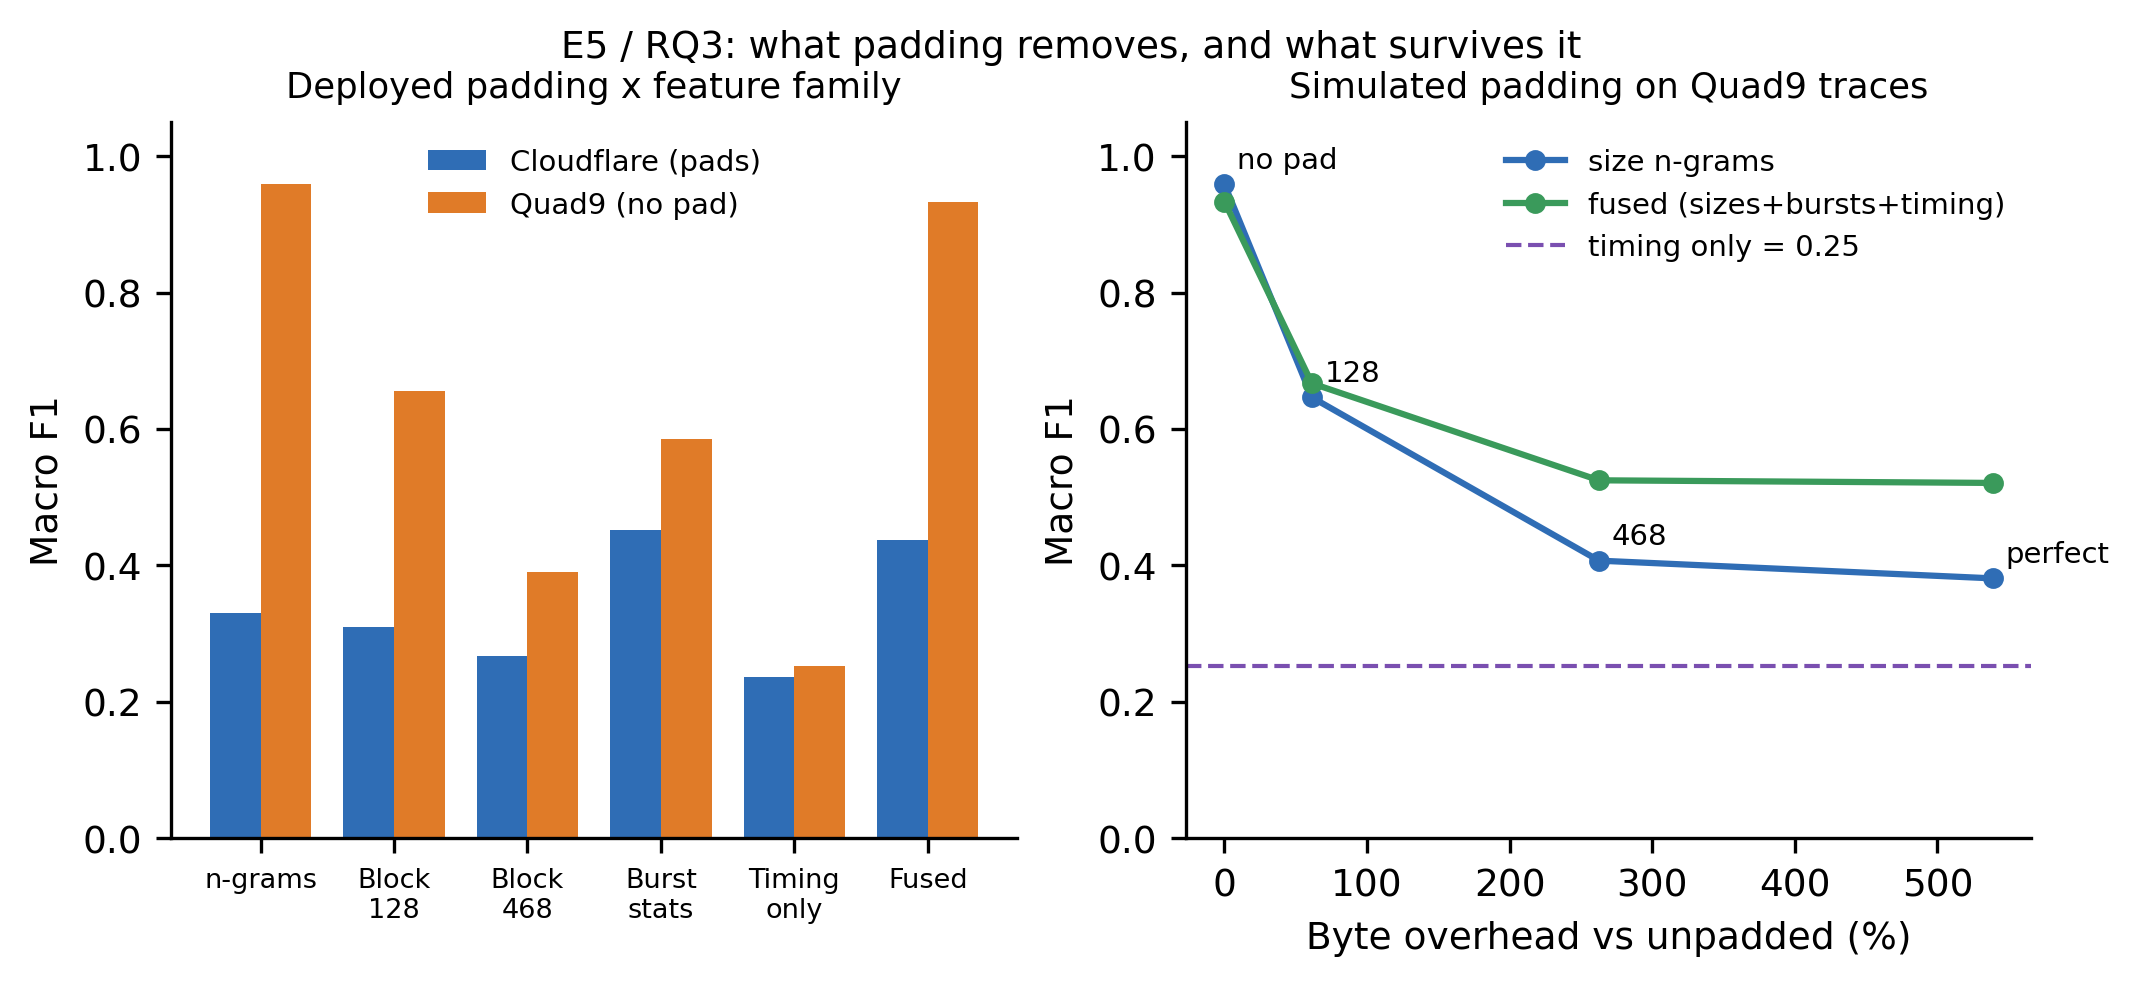
\includegraphics[width=0.88\textwidth]{figures/fig8_padding_effect.png}
\caption{Left: macro-\Fone{} by feature family on the padded and unpadded resolver. Right: padding simulated on Quad9 traces against byte overhead (dashed: timing only).}\label{fig:padding}
\end{figure}

\paragraph{Transfer and recovery (RQ2).} Figure~\ref{fig:transfer} is the transfer matrix of B1 over the 49 shared global sites (vimeo.com had too few valid Cloudflare traces). Within 2018 the attack transfers between places (Lausanne $\to$ Singapore 0.879; reverse 0.730), as Siby et al. found. Across eras every cell is at most 0.004 (chance 0.020), also between the two unpadded datasets, for burst statistics ($\le0.010$) and for block-index features ($\le0.041$); transfer also fails between the two 2026 resolvers (0.033, 0.021) and between Lausanne 2018 and 2019 (0.005). The representation, not the site, has changed: cloudflared over TLS~1.2 in 2018, Chrome over TLS~1.3 with padded queries in 2026. Fresh traces restore the attack (Figure~\ref{fig:recovery}): adding $k=1,2,5$ Cloudflare traces per site to the 2018 model gives 0.082, 0.171 and 0.336, against 0.076, 0.224 and 0.358 for the target traces alone, so old data adds nothing.

\begin{figure}[t]
\centering
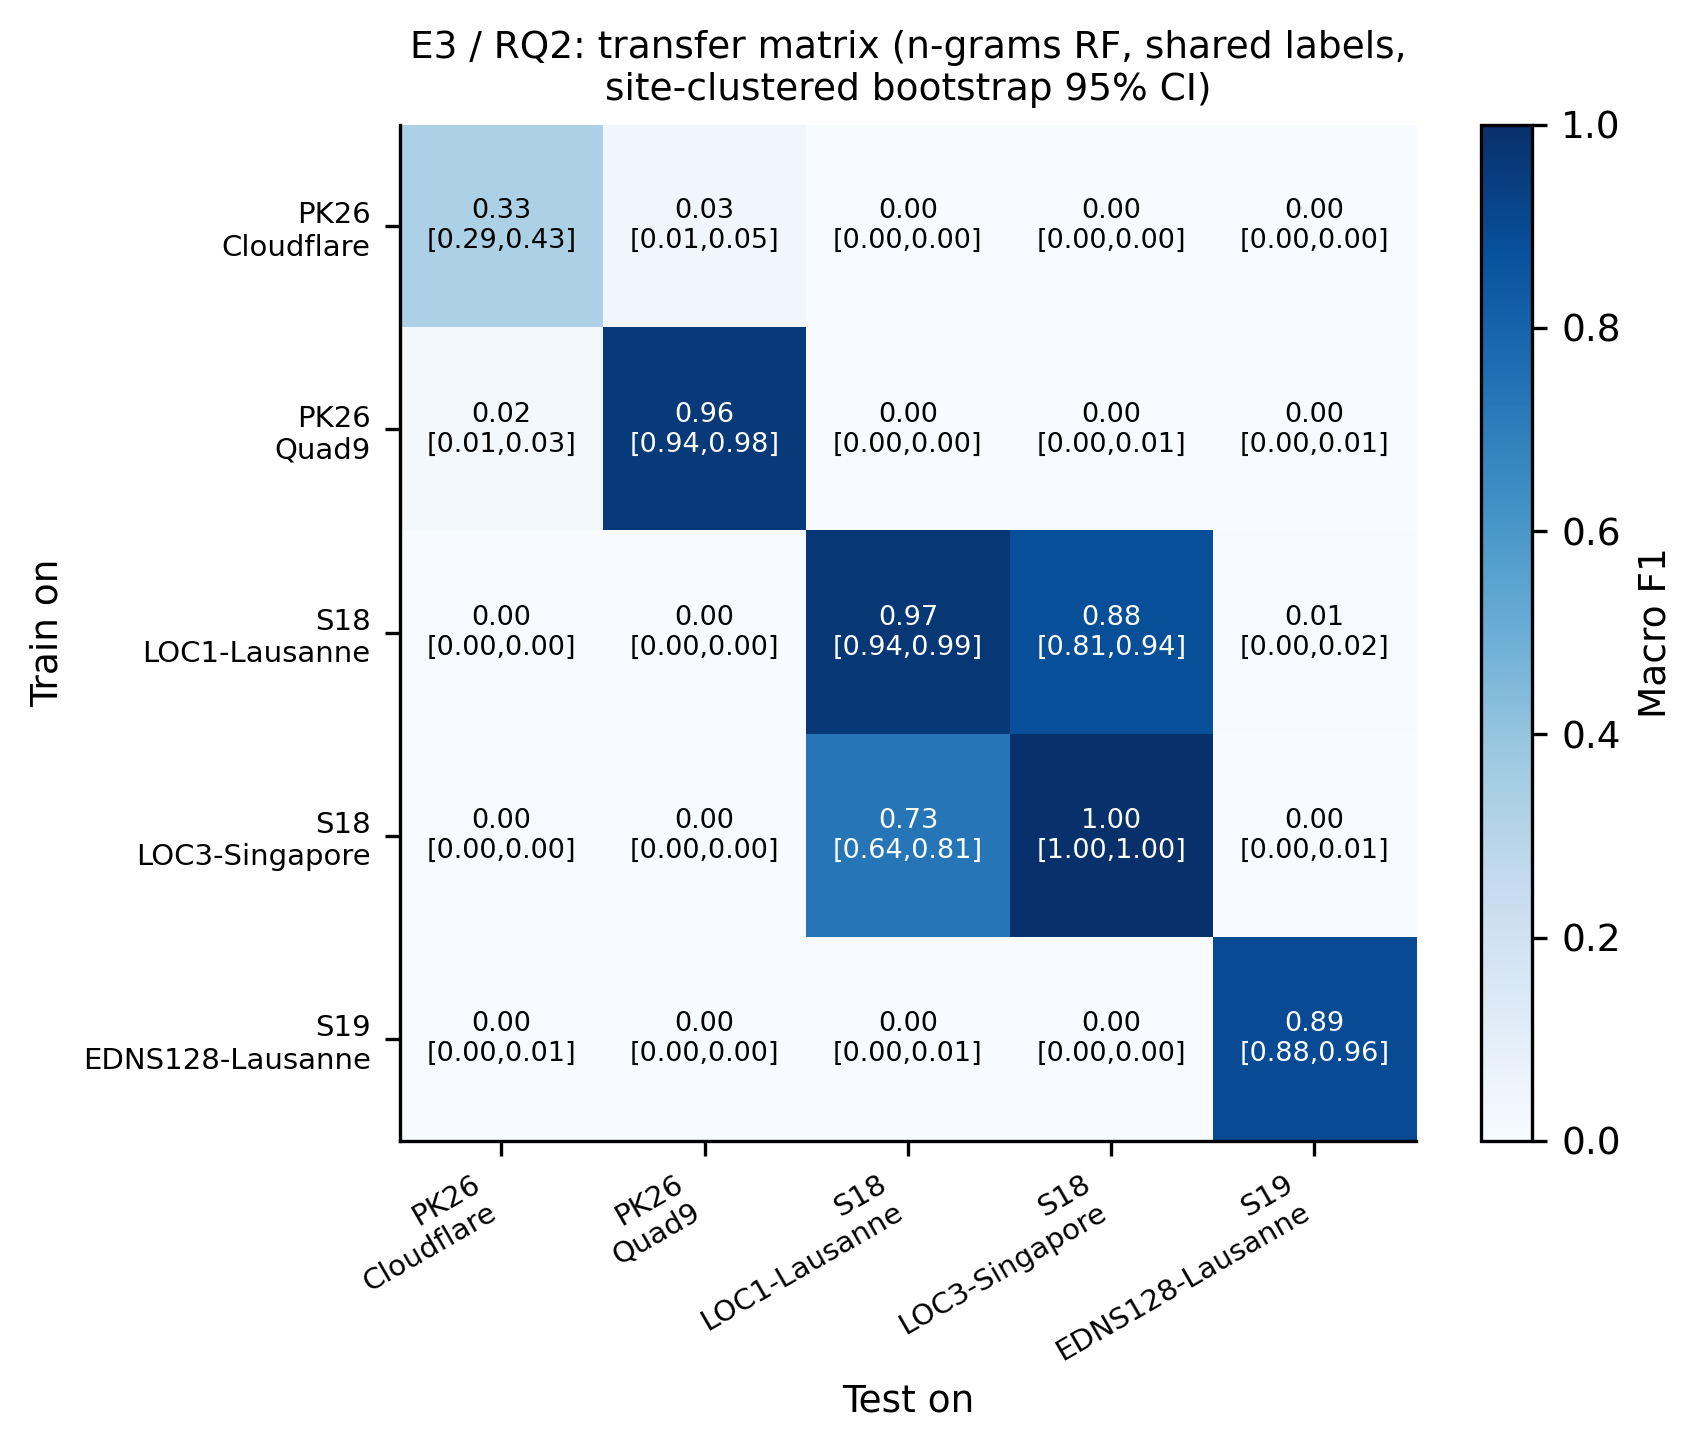
\includegraphics[width=0.62\textwidth]{figures/fig6_transfer_matrix.png}
\caption{Transfer matrix for B1 (rows train, columns test) with site-clustered 95\% confidence intervals. PK26: PK-DoH-2026; S18/S19: Siby's data.}\label{fig:transfer}
\end{figure}

%% ===================================================================== 6
\section{Comparison with Base Papers and the State of the Art}\label{sec:comparison}

\paragraph{Summary.} Table~\ref{tab:base} summarises the base papers: Siby et al.~\cite{siby2020} (reproduction target, B1), Moure-Garrido et al.~\cite{mouregarrido2026} (B5, F2), DoHFuse~\cite{zhang2026dohfuse} (timing features) and Shusterman et al.~\cite{shusterman2026} (recovery design).

\begin{table}[t]
\caption{Base papers (results as reported by the authors).}\label{tab:base}
\scriptsize\setlength{\tabcolsep}{3pt}
\begin{tabular*}{\textwidth}{@{\extracolsep\fill}L{0.12\textwidth}L{0.11\textwidth}L{0.14\textwidth}L{0.14\textwidth}L{0.08\textwidth}L{0.15\textwidth}L{0.15\textwidth}@{}}
\toprule
Paper & Problem & Method & Dataset & Metrics & Reported result & Key limitation \\
\midrule
Siby et al. 2020~\cite{siby2020} & WF on DoH & Size and burst n-grams, RF & 1,500 pages, 3 locations, 2018--19 & P, R, \Fone{} & \Fone{} 0.898; 0.430 at 468-B padding & Artefact differs from paper; never re-measured \\
Moure-Garrido et al. 2026~\cite{mouregarrido2026} & WF on DoQ & Burst statistics, RF & 986 sites, 9 nodes, one country & Acc., \Fone{} & Acc. 0.873; cross-node 53--81\% & One country; padding argued, not measured \\
DoHFuse 2026~\cite{zhang2026dohfuse} & WF on DoH/3 & Timing-only DMAG-LSTM & 449 sites $\times$ 100, US VPS & Acc., \Fone{} & 95.48\% (100 sites); size-only 67.39\% & One region; padding not audited \\
Shusterman et al. 2026~\cite{shusterman2026} & Drift & CNN+LSTM, retraining regimes & 100 sites, 26 weeks & Acc. & $>$95\% same week; $\approx$60\% after 26 weeks & One lab and browser; no variance \\
\botrule
\end{tabular*}
\end{table}

\paragraph{Quantitative comparison.} Table~\ref{tab:repro} compares the re-implementation with Siby et al. on their own data. The main configuration reproduces (0.893 against 0.898, TOST $p<0.001$), as do LOC2, LOC3, EDNS0-128 and perfect padding. Two artefact--paper discrepancies matter: the released code uses uni-grams only while the paper describes uni- and bi-grams (both reproduce), and perfect padding reproduces only when record direction is dropped too (0.043; 0.253 with direction), so the paper evidently set every packet to 825 bytes. EDNS0-468 comes out above the paper ($+0.078$); the released files do not say which 700 pages were used. On an identical 100-page setting (Table~\ref{tab:samedata}), n-grams lead and DF is last, as in the paper, but k-FP (0.913) clearly beats CUMUL (0.797).

\begin{table}[t]
\caption{Reproduction of~\cite{siby2020} on the released data (re-implemented in this work). \pub{} Published value. [pages $\times$ samples per page]. Verdict: \emph{yes} if $|\Delta|\le0.03$, \emph{partly} if $\le0.10$, otherwise \emph{no}.}\label{tab:repro}
\scriptsize\setlength{\tabcolsep}{2pt}
\begin{tabular*}{\textwidth}{@{\extracolsep\fill}lccccc@{}}
\toprule
Configuration & Published\pub{} & This work & $\Delta$ & TOST $p$ & Reproduced \\
\midrule
LOC1 [1,500$\times$60] & 0.898 & $0.893\pm0.001$ & $-0.005$ & $<0.001$ & yes \\
LOC1, all n-grams [1 fold] & 0.898 & 0.894 & $-0.004$ & -- & yes \\
LOC1, uni-grams only [1 fold] & 0.898 & 0.895 & $-0.003$ & -- & yes \\
LOC2 Leuven [1,500$\times$20] & 0.908 & $0.882\pm0.006$ & $-0.026$ & 0.169 & yes \\
LOC3 Singapore [1,500$\times$20] & 0.917 & $0.906\pm0.001$ & $-0.011$ & $<0.001$ & yes \\
EDNS0-128 [700$\times$60] & 0.691 & $0.703\pm0.005$ & $+0.012$ & 0.013 & yes \\
EDNS0-468 [700$\times$60] & 0.430 & $0.508\pm0.007$ & $+0.078$ & 0.997 & partly \\
Perfect, no direction [700$\times$60] & 0.066 & $0.043\pm0.002$ & $-0.023$ & 0.011 & yes \\
Perfect, with direction [700$\times$60] & 0.066 & $0.253\pm0.009$ & $+0.187$ & 0.999 & no \\
\botrule
\end{tabular*}
\end{table}

\paragraph{Methodological comparison and improvement.} B1 relies on exact sizes, so it is best when sizes are intact and weak when they are padded; B5 and DoHFuse discard sizes, which makes them robust to padding but weaker without it (B5: 0.596 on Quad9). M1 keeps all three views and lets the forest choose. Table~\ref{tab:improve} shows that M1 is never more than 0.025 below the best method but not the best everywhere: k-FP leads by 0.019 on Cloudflare (overlapping confidence intervals) and B1 by 0.025 on Quad9. Ablation A1 traces M1's gain over B1 to the burst statistics.

\begin{table}[t]
\caption{M1 against each re-implemented base method: absolute macro-\Fone{} change (relative change in brackets). Positive values favour M1.}\label{tab:improve}
\scriptsize\setlength{\tabcolsep}{3pt}
\begin{tabular*}{\textwidth}{@{\extracolsep\fill}lccc@{}}
\toprule
Condition & vs.\ B1 Siby~\cite{siby2020} & vs.\ B5 bursts~\cite{mouregarrido2026} & vs.\ B2 k-FP~\cite{hayes2016kfp} \\
\midrule
Cloudflare (deployed padding) & $+0.102$ ($+29.8\%$) & $+0.001$ ($+0.2\%$) & $-0.019$ ($-4.1\%$) \\
Quad9 (no padding) & $-0.025$ ($-2.6\%$) & $+0.327$ ($+54.9\%$) & $+0.280$ ($+43.5\%$) \\
Simulated 468-B padding & $+0.118$ ($+29.0\%$) & -- & -- \\
Simulated perfect padding & $+0.140$ ($+36.7\%$) & -- & -- \\
\botrule
\end{tabular*}
\end{table}

\paragraph{Fairness.} The reproduction uses the authors' data but evaluates 3 of 10 folds, uses 20 of 60 samples per page for LOC2 and LOC3 (if anything lowering \Fone{}) and prunes rare n-grams (unpruned: 0.894); for LOC2 the equivalence test is not significant. Comparisons with DoHFuse and Moure-Garrido et al. are indicative only, as they use other transports, regions and, for DoHFuse, ten times as many traces per site.

%% ===================================================================== 7
\section{Ablation Study}\label{sec:ablation}

\begin{table}[t]
\caption{Ablation A1: feature groups (macro-\Fone{}, 5 splits).}\label{tab:a1}
\scriptsize\setlength{\tabcolsep}{2pt}
\begin{tabular*}{\textwidth}{@{\extracolsep\fill}lcc|lcc@{}}
\toprule
Features & Cloudflare & Quad9 & Features & Cloudflare & Quad9 \\
\midrule
Size uni-grams & 0.303 & \textbf{0.978} & F1 + F2 (bursts) & 0.444 & 0.932 \\
Size uni+bi-grams & 0.374 & 0.969 & F1 + F5 (timing) & 0.357 & 0.951 \\
Burst uni+bi-grams & 0.137 & 0.459 & F1 + F2 + F5 (M1) & 0.437 & 0.933 \\
F1 (B1) & 0.331 & 0.959 & F2 + F5 (no sizes) & \textbf{0.470} & 0.575 \\
F1 + tri-grams & 0.341 & 0.934 & & & \\
\botrule
\end{tabular*}
\end{table}

\paragraph{A1: feature groups.} Table~\ref{tab:a1} removes and adds feature families. On Quad9, size n-grams carry the attack and tri-grams add nothing. On Cloudflare the picture reverses: adding burst statistics to the n-grams raises \Fone{} from 0.331 to 0.444, timing raises it only to 0.357, timing on top of the bursts adds nothing (0.437), and dropping the size n-grams even helps slightly (0.470). Under padding, a page is identified by how many exchanges it makes and how they are grouped, not by fine-grained timing.

\paragraph{A2--A4: prefix, budget and world size.} On Quad9 (Figure~\ref{fig:a234}) the first 50 records give 0.057 but the first 100 give 0.958, as the opening records are browser start-up lookups common to all sites. The attack is still data-limited (1, 2 and 5 traces per site: 0.328, 0.693, 0.917), and accuracy falls as the closed world grows (Cloudflare: 0.743 at 10 sites, 0.367 at 98), which is why EDNS0-468 over all 1,500 labels gave only 0.330 (Table~\ref{tab:sens}).

\paragraph{A5--A7: label set, curation and CNN components.} Pakistani and global sites are identified equally well (Quad9: 0.953 and 0.959; Cloudflare: 0.430 and 0.427). Removing the bot-challenge sites leaves Quad9 unchanged and raises Cloudflare from 0.331 to 0.390, so the padded results reported here are conservative. In M2, removing the squeeze-and-excitation block helps (Quad9: 0.354 to 0.379; 2018 data: 0.680 to 0.788) while removing the timing channel hurts (0.354 to 0.269): channel attention does not help on short DNS traces at this sample size.

%% ===================================================================== 8
\section{Discussion}\label{sec:discussion}

\paragraph{Why it works and what it means.} Each page triggers its own set of lookups, whose number, order and sizes vary little between visits. Padding removes the sizes but not the number or grouping of the lookups, so burst features and M1 survive it: on DNS traces, what survives size-only defences~\cite{gong2026wfcat,bushart2020} is coarse burst structure rather than fine timing. For users, protection depends on an invisible combination of client and resolver (a Chrome user is padded on Cloudflare or Google but not on Quad9, NextDNS, DNS.SB or AliDNS), which resolvers could remove by padding unconditionally, as OpenDNS does. For researchers, models are as short-lived as client software and must be retrained, not reused.

\paragraph{Strengths.} The two 2026 conditions share sites, network, browser, week and collection script and differ only in the resolver and hence its padding. Padding is measured from decrypted replies rather than assumed, the reproduction is judged on the authors' own data against a tolerance fixed in advance, and every in-domain result carries its spread over repeated splits.

\paragraph{Failure cases.} Under deployed padding, 42 of 98 sites are never identified (Figure~\ref{fig:cdf}). M1 trails k-FP on padded traffic (0.444 against 0.463) and B1 on unpadded traffic (by 0.025); M2 is weak at this sample size, and its attention block lowers accuracy. EDNS0-468 is only partly reproduced, and perfect padding matches the paper only under a corrected reading of the setup.

\paragraph{Research gaps.} Of the four gaps from the literature review, three are closed (Table~\ref{tab:gaps}, Appendix~\ref{app:extra}): the 2020 attack is re-measured, deployed padding is tied to attack accuracy, and results carry stated uncertainty under a pre-registered criterion. The location gap is only partly closed: the change of client, TLS and padding between eras hides any location effect, so regional CDN steering was neither confirmed nor ruled out.

\paragraph{Limitations and threats to validity.} With 10 traces per site and 100 sites, absolute values are lower bounds (A3) and the neural models are under-trained. All 2026 data come from one Wi-Fi network and Chrome~157; crawls are more regular than real browsing~\cite{jansen2026gtt23,deng2026}, and an open world would lower all numbers. Only 3 of 10 reproduction folds were evaluated, and parallel workers may add timing noise (each capture is filtered to one resolver address, so traces cannot mix). McNemar tests, multiple-comparison correction and a confusion-cluster analysis were planned but not done.

%% ===================================================================== 9
\section{Conclusion and Future Work}\label{sec:conclusion}

The 2020 attack on encrypted DNS reproduces within a pre-registered tolerance and in 2026 remains effective against an unpadded resolver (macro-\Fone{} 0.948). Deployed padding reduces it to 0.342, but only where client and resolver both pad, and a fused model of sizes, bursts and timing recovers part of the loss (0.444). Models from 2018--19 do not transfer to 2026, but a few fresh traces per site rebuild the attack. Future work should add traces per site, a mobile network and a second country to isolate location, track padding over time and across browsers, and evaluate defences that also shape the number and timing of exchanges.

\backmatter

\bmhead{Acknowledgements}
The authors thank Siby et al. for releasing their code and data~\cite{sibycode}.

\section*{Declarations}
\begin{itemize}
\item \textbf{Funding:} none. \textbf{Conflict of interest:} none. \textbf{Ethics:} not applicable; all traffic was generated by the authors' own crawler to public resolvers, and no third-party or user traffic was captured.
\item \textbf{Data and code availability:} PK-DoH-2026, all code, result files and the paper source are available at \url{https://github.com/muhammadkaif654/pk-doh-2026}, with a README for regenerating every table and figure; Siby et al.'s data are at~\cite{sibycode}.
\item \textbf{Use of AI tools:} The authors used Claude (Anthropic) to help write and debug analysis code and to draft and edit the manuscript. All experiments ran with the authors' code on the authors' machine, every number was checked against the result files, and the authors take full responsibility for the content.
\item \textbf{Author contributions:} M.K.: capture pipeline, resolver setup, padding audit. S.A.: features, models, evaluation. Both: reproduction, analysis, writing.
\end{itemize}

%% Appendix floats are in the order in which the main text first cites them.
\begin{appendices}

\section{Supplementary material}\label{app:extra}

\begin{algorithm}[h]
\caption{Streaming random forest (identical output, bounded memory)}\label{alg:forest}
\begin{algorithmic}[1]
\Require training set $(X,y)$, test set $X'$, number of trees $N_T$, batch size $m$, seed $r$
\State $S\gets\mathbf{0}_{|X'|\times K}$
\For{$j=0,m,\dots,N_T-m$}
  \State grow trees $j,\dots,j+m-1$ on bootstrap samples of $(X,y)$ (seeds $r+j,\dots$)
  \State $S\gets S+\sum$ of their predicted probabilities on $X'$; free the trees
\EndFor
\State \Return $S/N_T$
\end{algorithmic}
\end{algorithm}

\begin{table}[h]
\caption{Changes from the planned methodology.}\label{tab:deviations}
\scriptsize
\begin{tabular*}{\textwidth}{@{\extracolsep\fill}L{0.22\textwidth}L{0.22\textwidth}L{0.48\textwidth}@{}}
\toprule
Item & Plan & What was done and why \\
\midrule
DoT, GOOGLE/CLOUD sets & Reproduce & Not released; DoT covered by the audit only \\
Released code & Run unchanged & Python 2 and uni-grams only; ported, both feature sets reported \\
Forest memory & Standard RF & About 100\,GB needed; streaming forest (Algorithm~\ref{alg:forest}) \\
n-gram vocabulary, folds & All n-grams, 10 folds & Pruned (check row unpruned); first 3 folds, for compute \\
Countermeasure sets & As released & Paper's 700 $\times$ 60 configuration; 1,500-label runs in Table~\ref{tab:sens} \\
Traces per site; network & 30; Wi-Fi and 4G & 10 per site; 4G not collected, replaced by the resolver contrast \\
TLS 1.3 records & Not anticipated & Handshake and tickets removed (Algorithm~\ref{alg:extract}) \\
Recovery budget; F5 slots & $k\le20$; 10--20\,ms & $k\le5$ (half of 10 traces held out); 250\,ms, as traces last about 10\,s \\
Statistics, error analysis & McNemar, Holm, Cliff's delta, confusion clusters & Not done; Wilcoxon, bootstrap, TOST and per-site \Fone{} instead \\
\botrule
\end{tabular*}
\end{table}

\begin{table}[h]
\caption{Implementation details and hyperparameters.}\label{tab:impl}
\scriptsize
\begin{tabular*}{\textwidth}{@{\extracolsep\fill}L{0.20\textwidth}L{0.74\textwidth}@{}}
\toprule
Item & Setting \\
\midrule
Random forests & $N_T=100$ fully grown trees, $\sqrt{d}$ features per split, bootstrap, probability averaging; B5: 200 trees, balanced weights; n-grams kept if in $\ge3$ training traces \\
SVM (B3) & RBF kernel, $C=1000$ \\
Neural (B4, M2) & AdamW, learning rate $2\times10^{-3}$ ($10^{-3}$ for DF), cosine schedule, batch 128, label smoothing 0.05, $\le$40 epochs, early stopping on 10\% of training data, shift augmentation $\pm3$ \\
Features & $\tau=25$\,ms (F2); 200 records (F3); $\beta\in\{128,468\}$ (F4); 20 slots $\times$ 250\,ms, 8 bins (F5) \\
Random seeds & Splits: stratified, \texttt{random\_state}=0 (E1 10-fold; E2--E5 repeated 80/20); model seed = fold or split index $0,1,2,\dots$; site-clustered bootstrap seed 0 \\
Capture & Chrome 157 headless, Selenium 4.52, ChromeDriver 157, dumpcap/tshark 4.6.8; 30\,s timeout, 5\,s idle; QUIC off \\
Environment & Intel i7-13620H (10 cores), 16\,GB RAM, no GPU, Windows 11; Python 3.14, scikit-learn 1.8, PyTorch 2.11 (CPU), NumPy 2.4, pandas 3.0, SciPy 1.17 \\
\botrule
\end{tabular*}
\end{table}

\begin{table}[h]
\caption{All methods on an identical setting: 100 LOC1 pages $\times$ 60 traces, 3 splits (2 for neural models). \pub{} Siby et al. at 1,500 pages, for reference.}\label{tab:samedata}
\scriptsize
\begin{tabular*}{\textwidth}{@{\extracolsep\fill}lcccc@{}}
\toprule
Method & Macro-\Fone{} (this work) & Acc. & Top-5 & Published\pub{} \\
\midrule
B1 n-grams + RF & $0.961\pm0.008$ & 0.961 & 0.987 & 0.87 \\
B2 k-FP & $0.913\pm0.006$ & 0.913 & 0.957 & 0.74 \\
B3 CUMUL & $0.797\pm0.003$ & 0.801 & 0.927 & 0.75 \\
B4 DF & $0.593\pm0.008$ & 0.611 & 0.911 & 0.51 \\
B5 Burst-stats RF & $0.904\pm0.009$ & 0.905 & 0.958 & -- \\
M1 Fused RF (proposed) & $0.959\pm0.005$ & 0.959 & 0.986 & -- \\
M2 1D-CNN + SE (proposed) & $0.680\pm0.045$ & 0.693 & 0.917 & -- \\
\botrule
\end{tabular*}
\end{table}

\begin{table}[h]
\caption{Sensitivity runs over all 1,500 released page labels (not part of the verdicts).}\label{tab:sens}
\scriptsize
\begin{tabular*}{\textwidth}{@{\extracolsep\fill}lccc@{}}
\toprule
Configuration & Published\pub{} & This work & $\Delta$ \\
\midrule
EDNS0-128 [1,500 $\times$ 20] & 0.691 & $0.584\pm0.006$ & $-0.107$ \\
EDNS0-468 [1,500 $\times$ 10] & 0.430 & $0.330\pm0.006$ & $-0.100$ \\
Perfect, direction kept [1,500 $\times$ 60] & 0.066 & $0.200\pm0.003$ & $+0.134$ \\
\botrule
\end{tabular*}
\end{table}

\begin{table}[h]
\caption{Research gaps and whether this work closes them.}\label{tab:gaps}
\scriptsize
\begin{tabular*}{\textwidth}{@{\extracolsep\fill}L{0.34\textwidth}L{0.48\textwidth}L{0.10\textwidth}@{}}
\toprule
Gap & Evidence & Status \\
\midrule
2020 DoH attack never re-measured & Reproduction within tolerance; 2026 re-measurement (Tables~\ref{tab:repro}, \ref{tab:e2}) & closed \\
Transfer untested outside one country & First South Asian dataset and cross-era matrix; location effect hidden by client change & partly \\
Padding never tied to deployed accuracy & 11-resolver audit, single-factor contrast, simulation (Table~\ref{tab:audit}, Figure~\ref{fig:padding}) & closed \\
Thin statistics, no reproduction criterion & Pre-registered tolerance, TOST, repeated splits, clustered bootstrap & closed \\
\botrule
\end{tabular*}
\end{table}

\begin{figure}[h]
\centering
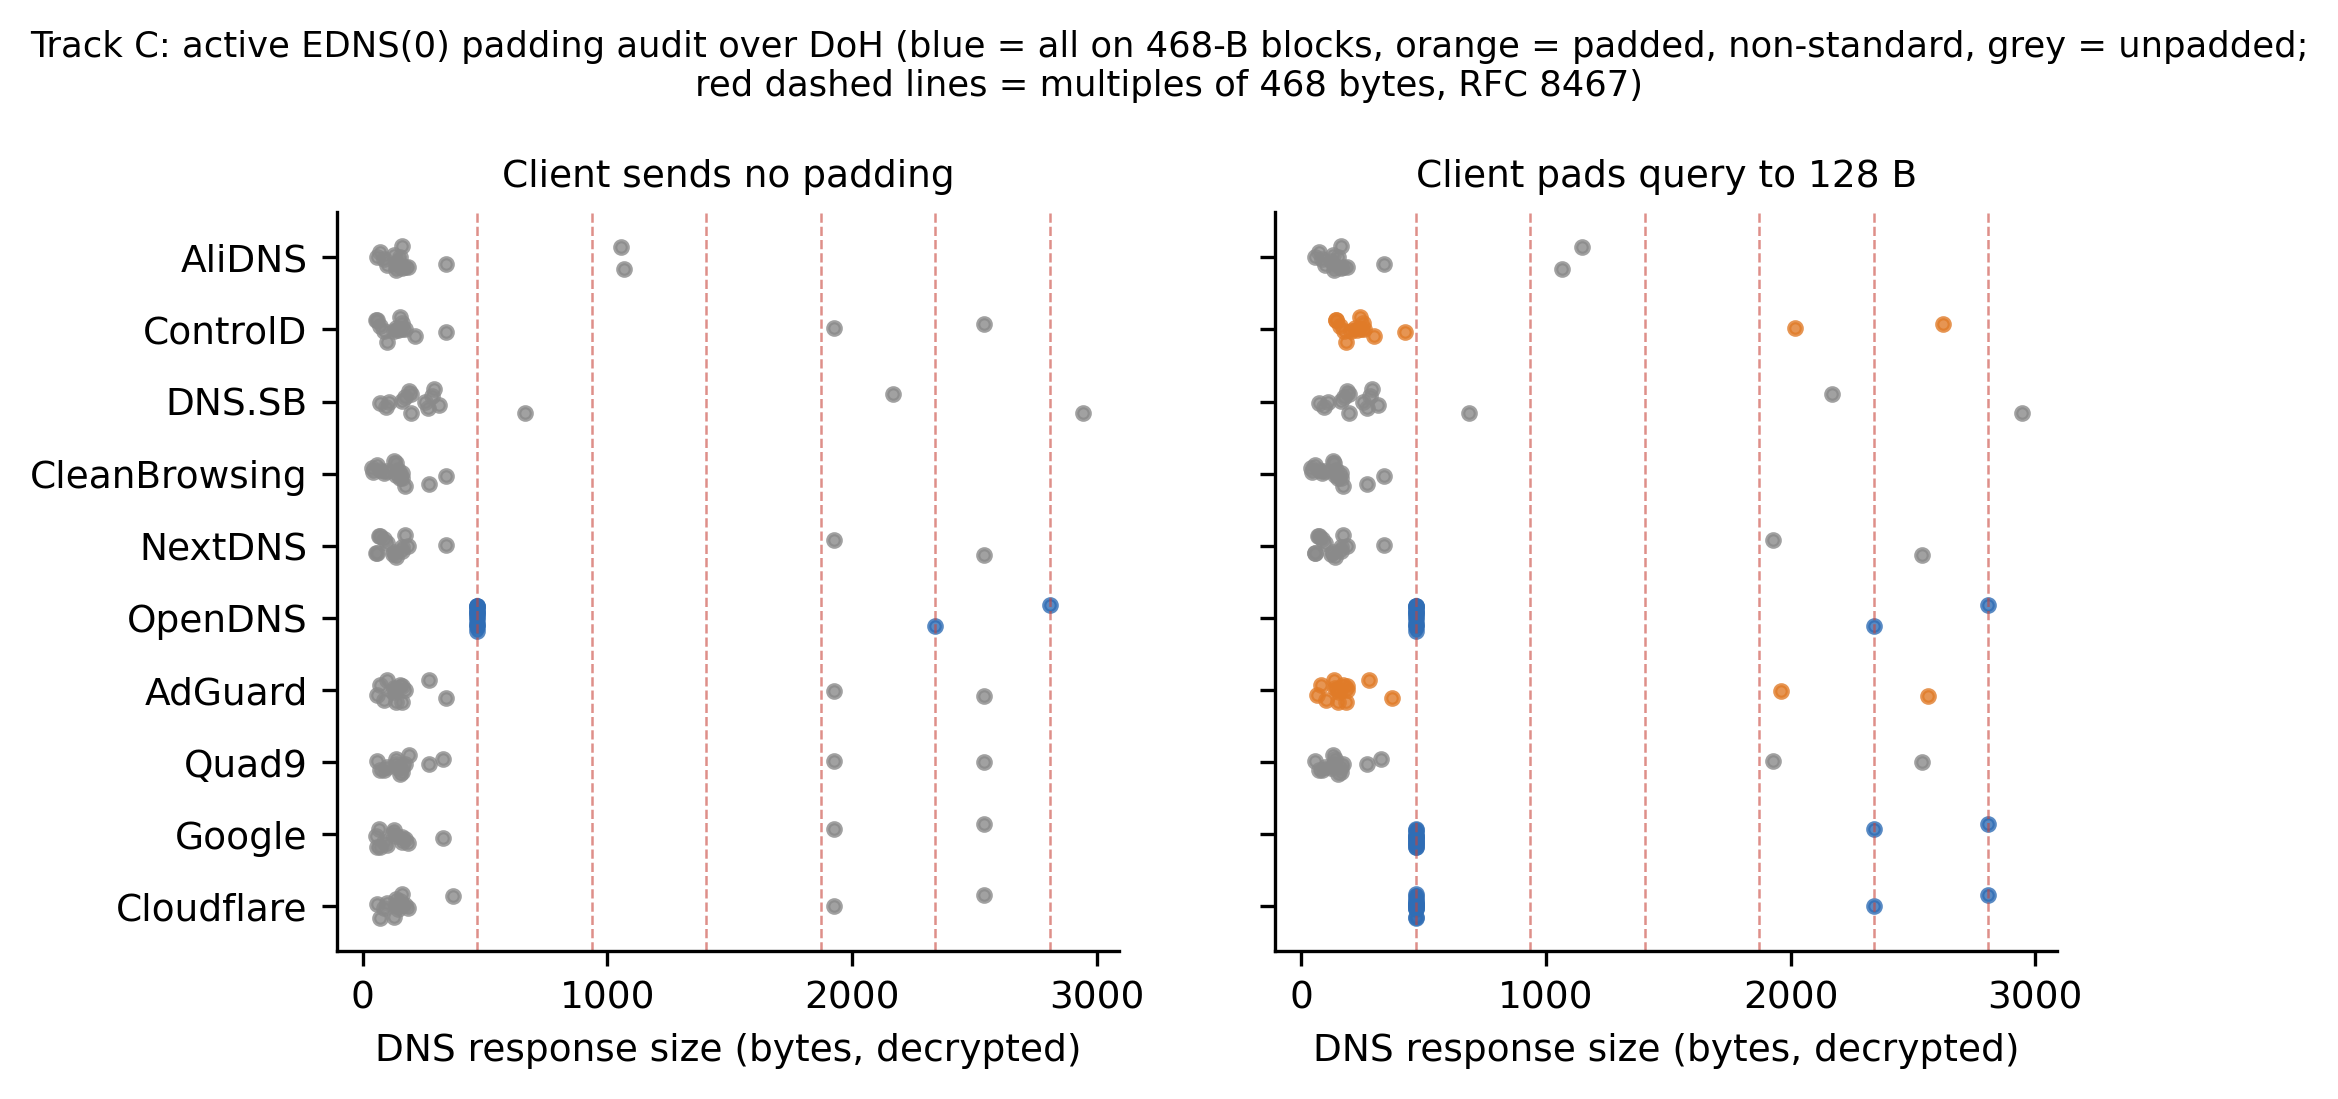
\includegraphics[width=\textwidth]{figures/fig3_padding_audit.png}
\caption{Decrypted DoH response sizes per resolver, without (left) and with (right) a padded client query; padded replies sit on multiples of 468 bytes.}\label{fig:audit}
\end{figure}

\begin{figure}[h]
\centering
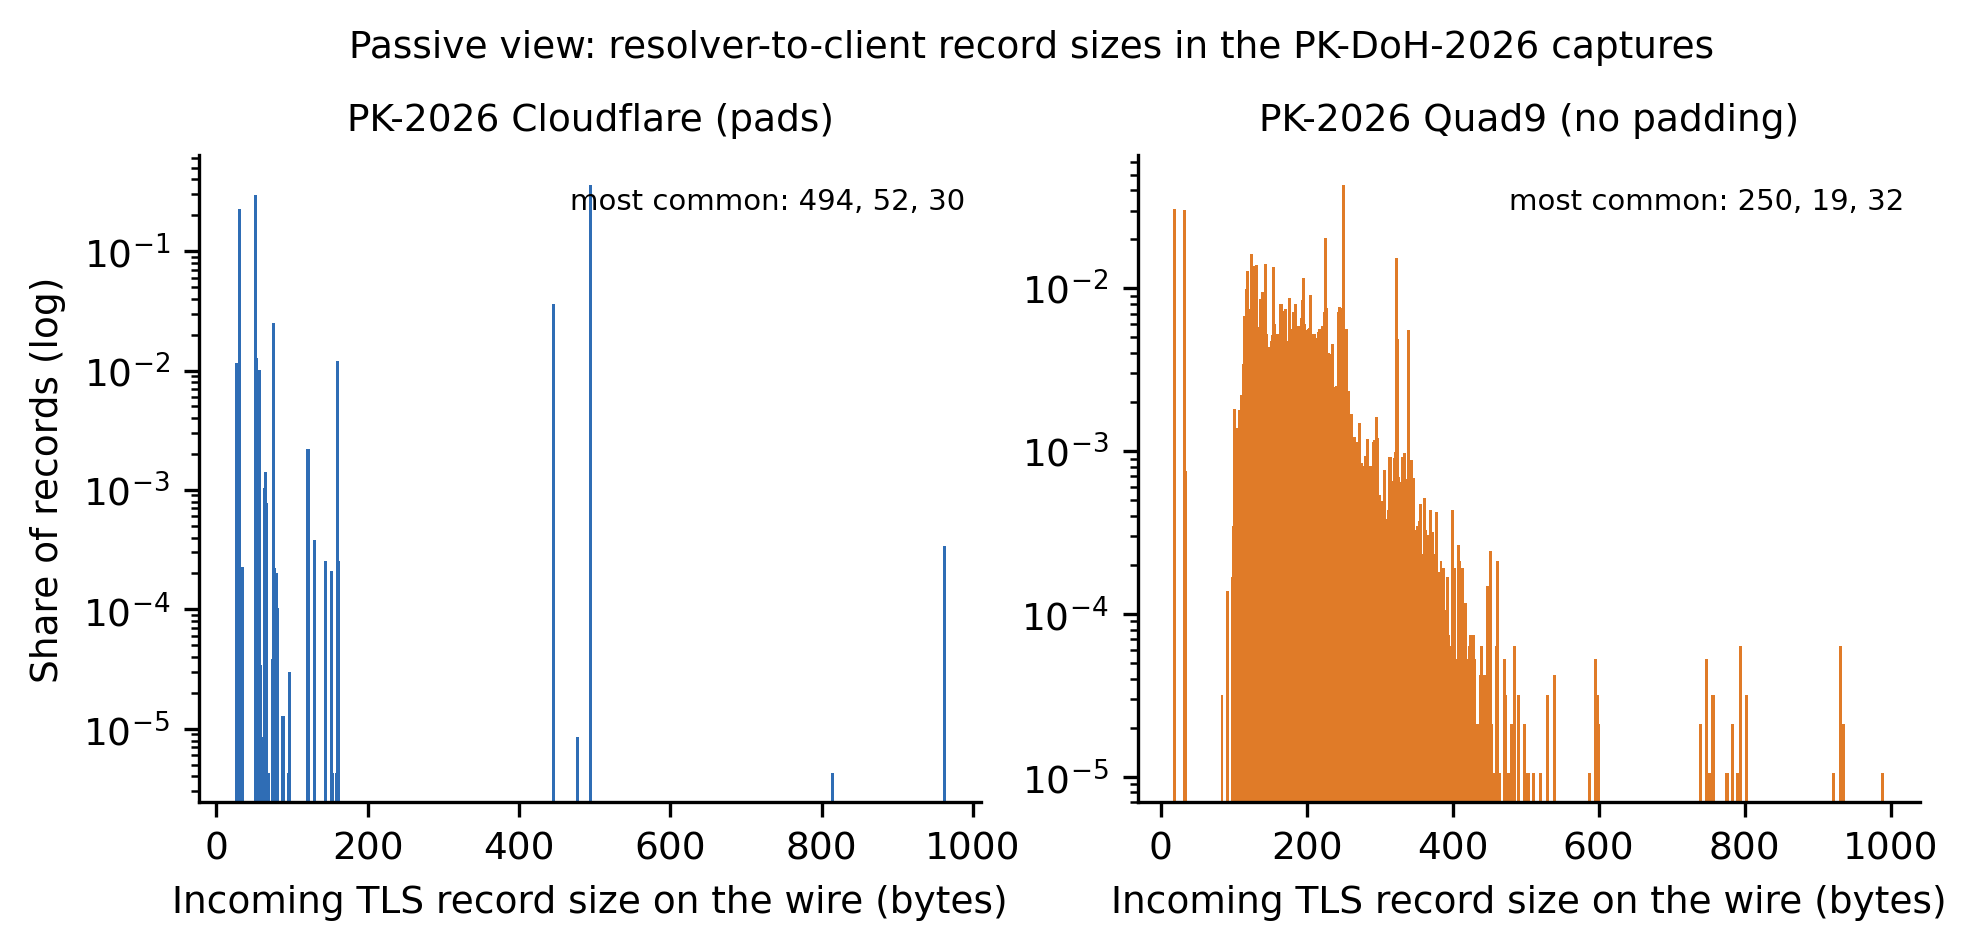
\includegraphics[width=\textwidth]{figures/fig4_wire_histograms.png}
\caption{Qualitative example: resolver-to-client record sizes on the wire. Cloudflare collapses onto a few sizes (494 bytes is one padded 468-byte message plus framing); Quad9 spreads over hundreds.}\label{fig:wire}
\end{figure}

\begin{figure}[h]
\centering
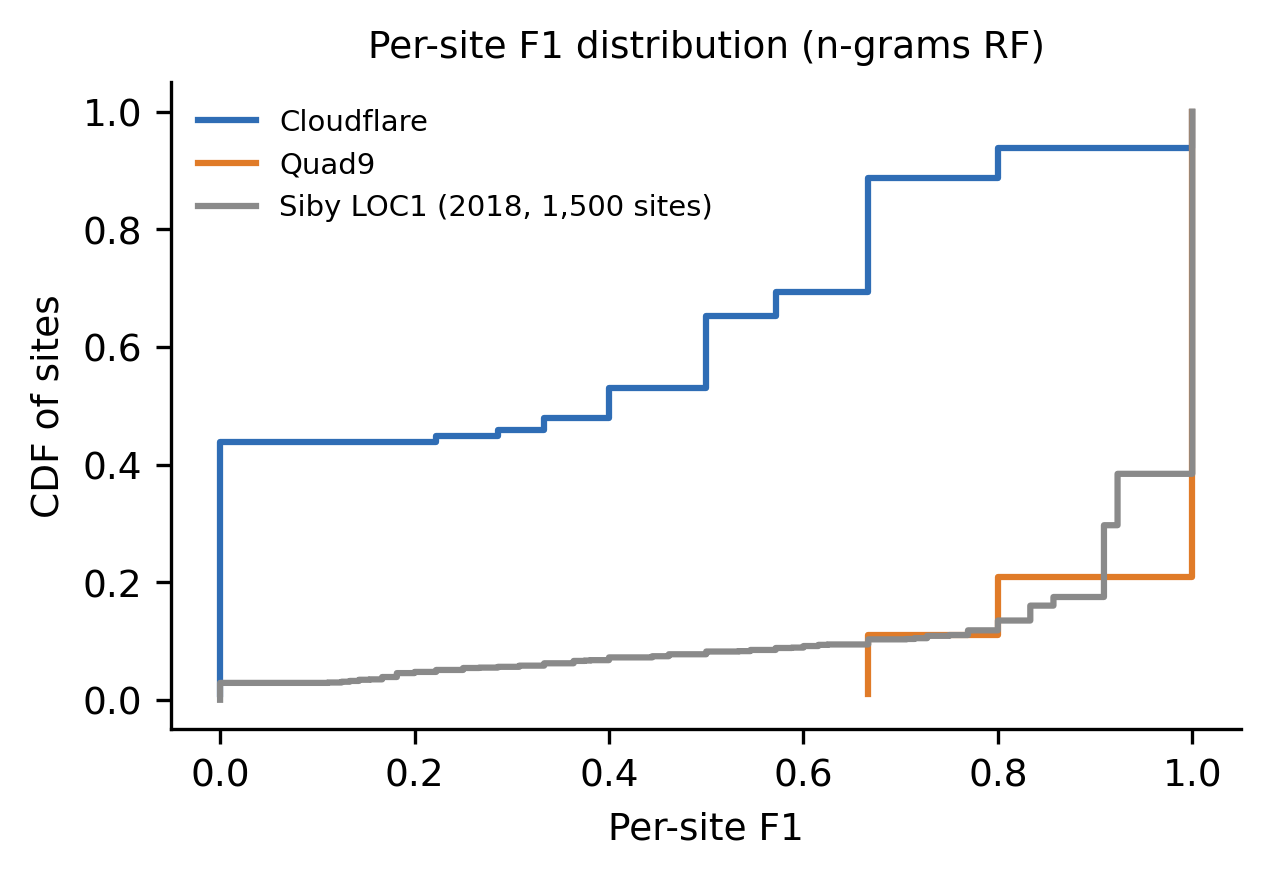
\includegraphics[width=0.7\textwidth]{figures/fig11_per_site_cdf.png}
\caption{Distribution of per-site \Fone{} for B1: under padding many sites are never identified, a minority remain easy to identify.}\label{fig:cdf}
\end{figure}

\begin{figure}[h]
\centering
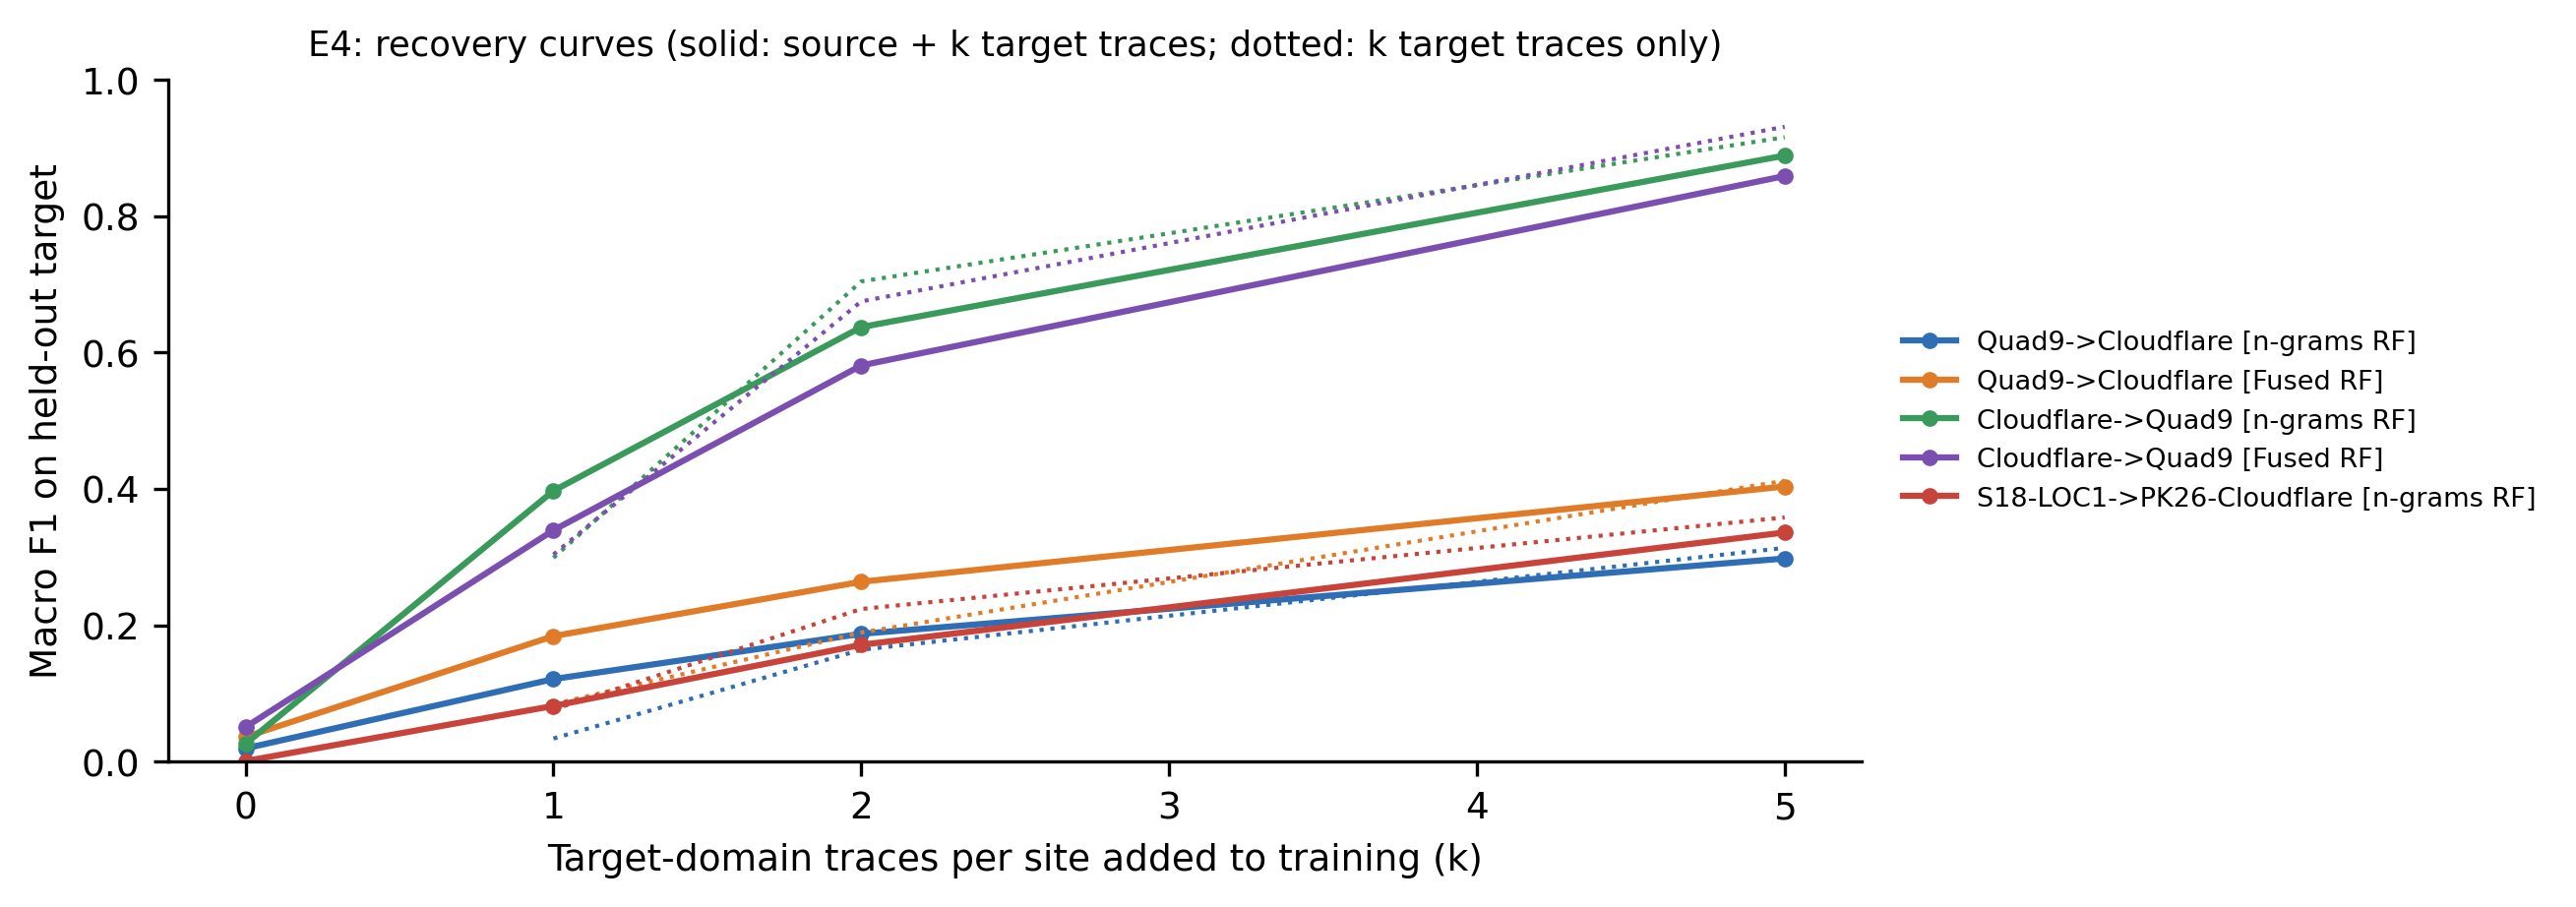
\includegraphics[width=\textwidth]{figures/fig7_recovery.png}
\caption{Recovery: macro-\Fone{} on held-out target traces with $k$ target traces per site added to the source data (solid) or alone (dotted).}\label{fig:recovery}
\end{figure}

\begin{figure}[h]
\centering
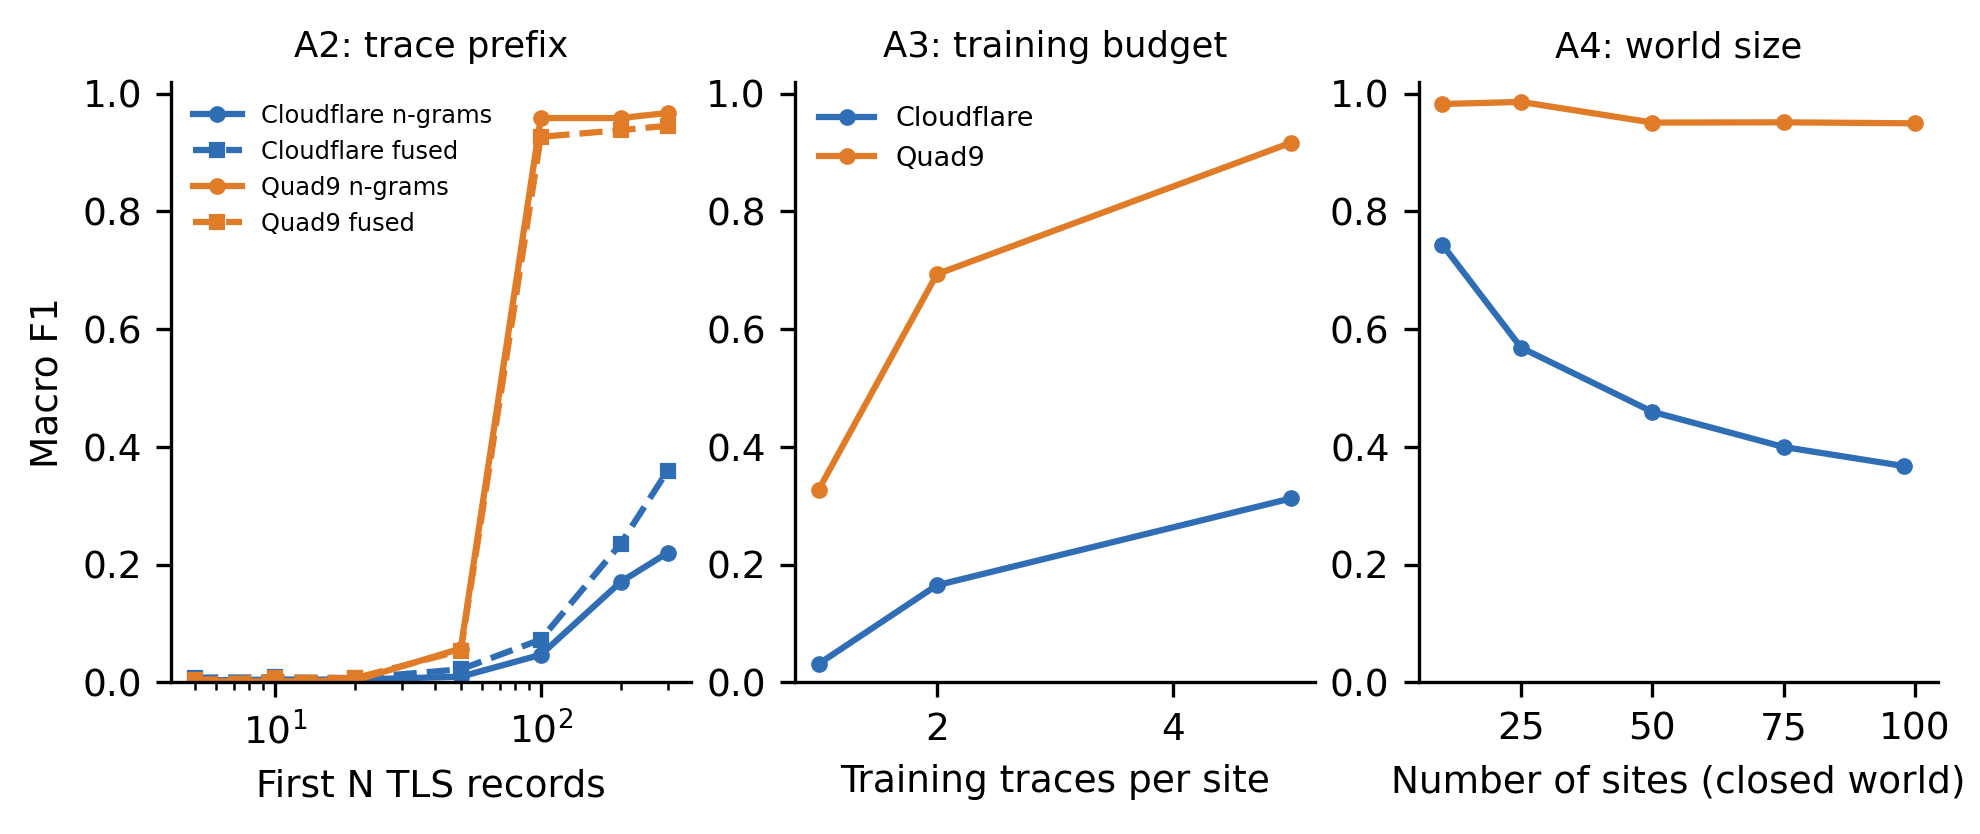
\includegraphics[width=\textwidth]{figures/fig10_ablation_curves.png}
\caption{Ablations A2 (first $N$ records), A3 (training traces per site) and A4 (number of sites).}\label{fig:a234}
\end{figure}

\clearpage
\end{appendices}

\bibliography{references}

\end{document}
